%驻波的简要报告

\documentclass[UTF8]{ctexart}

\title{电子技术基础实验第六周实验报告}

\author{王磊\quad2022012972}

\date{\today}

\usepackage{geometry}
\geometry{a4paper,scale=0.8}

\usepackage{graphicx}
\usepackage{subfigure}
\usepackage{float}

\usepackage{amsmath}

\usepackage{listings}
\usepackage{xcolor}
\usepackage{framed}
\lstdefinestyle{verilogStyle}{
    language=verilog,
    basicstyle=\ttfamily,
    keywordstyle=\color{blue},
    commentstyle=\color{green},
    stringstyle=\color{red},
    numbers=left,
    numberstyle=\tiny\color{gray},
    breaklines=true,
    showstringspaces=false,
    columns = fixed,
    basewidth = 0.5em,
    captionpos=b,
}
\newcommand{\subsubsubsection}[1]{\paragraph{#1}\mbox{}\\}
\setcounter{secnumdepth}{4} % how many sectioning levels to assign numbers to
\setcounter{tocdepth}{4} % how many sectioning levels to show in ToC
%设置段落间距
\setlength{\parskip}{0.5em}
%令小标题左对齐
\CTEXsetup[format={\Large\bfseries}]{section}
%首行不缩进
\setlength{\parindent}{0pt}
\begin{document}
\maketitle
%小标题
\section{task1\_3}
\subsection{模块设计}
\subsubsection{上升沿检测模块}
\subsubsubsection{模块代码}
\begin{framed}
    \begin{lstlisting}[language=verilog,style=verilogStyle]
    reg pulse1_1, pulse1_2, pulse1_3;
    always @(posedge clk or posedge reset) begin
        if(reset)
        begin 
            pulse1_1 <= 1'b0;
            pulse1_2 <= 1'b0;
            pulse1_3 <= 1'b0;
        end
        else
        begin
            pulse1_1 <= button_io1;
            pulse1_2 <= pulse1_1;
            pulse1_3 <= pulse1_2;
        end
    end
    wire button1_negedge = ~pulse1_2 & pulse1_3;
    wire button1_posedge = pulse1_2 & ~pulse1_3;
\end{lstlisting}
\end{framed}
本模块采取基本的状态机设计,用三个寄存器存储三个时刻的按键状态,通过异或门检测下降沿和上升沿。

三个按键独立设计,故有三个检测模块,实际上可以通过一个模块解决,可以优化代码臃肿度。
\subsubsubsection{模块仿真}
\begin{figure}[H]
    \centering
    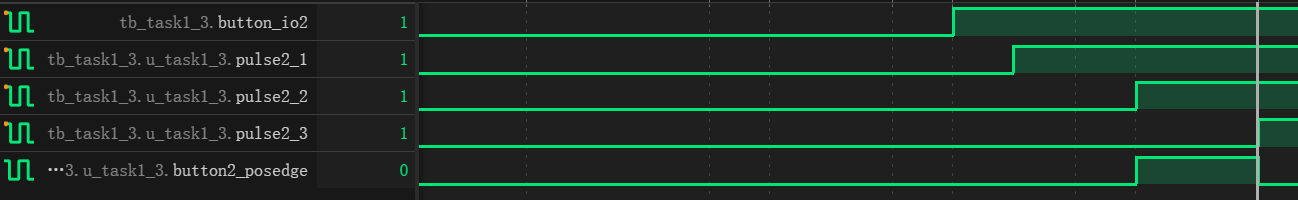
\includegraphics[width=0.8\textwidth]{task1_3_1.png}
    \caption{下降沿检测模块仿真}
\end{figure}
\subsubsection{按键检测模块}
\subsubsubsection{模块代码}
\begin{framed}
    \begin{lstlisting}[language=verilog,style=verilogStyle]
reg [31:0] cnt;
always @ (posedge clk or posedge reset)begin
    if(reset) begin
        cnt <= 32'b0;
    end
    else if(delay_flag) begin
        if(cnt == `CNT_MAX-1)
            cnt <= 32'b0;
        else begin
            cnt <= cnt + 32'b1;
        end
    end
end


reg delay_flag; 
always @(posedge clk or posedge reset) begin
    if(reset) begin
        delay_flag <= 1'b0;
    end
    else if(button1_posedge || button2_posedge || button3_posedge) begin
        delay_flag <= 1'b1;
    end
    else if(cnt == `CNT_MAX-1) begin
        delay_flag <= 1'b0;
    end
end
\end{lstlisting}
\end{framed}
逻辑为当检测到按键上升沿时,置延时标志位,同时开始计数,当计数到达设定值时,清除标志位,延时结束。延时的作用是消除机械按键的抖动,保证按键检测稳定。消抖后即可读取按键状态,进行相应操作。
\begin{framed}
    \begin{lstlisting}[language=verilog,style=verilogStyle]
reg button1_state, button2_state, button3_state;
always @(posedge clk or posedge reset) begin
    if(reset) begin
        button1_state <= 1'b0;
        button2_state <= 1'b0;
        button3_state <= 1'b0;
    end
    else if(cnt == `CNT_MAX-1) begin
        button1_state <= button_io1;
        button2_state <= button_io2;
        button3_state <= button_io3;
    end
    else begin
        button1_state <= 1'b0;
        button2_state <= 1'b0;
        button3_state <= 1'b0;
    end
end
    \end{lstlisting}
\end{framed}

\subsubsubsection{模块仿真}
\begin{figure}[H]
    \centering
    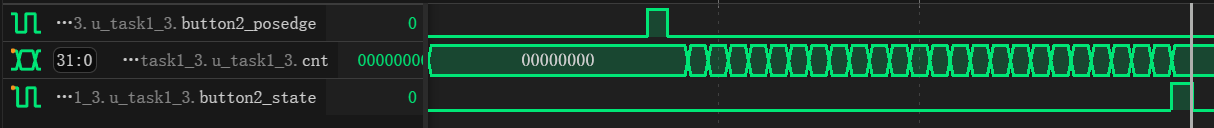
\includegraphics[width=0.8\textwidth]{task1_3_2.png}
    \caption{按键消抖模块仿真}
\end{figure}
可以看出检测到按键上升沿后经计数器延时到按键状态稳定时,才读取按键状态。
\subsubsection{流水灯模块}
\subsubsubsection{模块代码}
首先通过按键状态确定流水灯状态:
\begin{framed}
    \begin{lstlisting}[language=verilog,style=verilogStyle]
reg led_state1_flag, led_state2_flag, led_state3_flag;
always @(posedge clk or posedge reset) begin
    if(reset) begin
        led_state1_flag <= 1'b0;
        led_state2_flag <= 1'b0;
        led_state3_flag <= 1'b0;
    end
    else if(button1_state) begin
        led_state1_flag <= 1'b1;
        led_state2_flag <= 1'b0;
        led_state3_flag <= 1'b0;
    end     
    else if(button2_state) begin
        led_state1_flag <= 1'b0;
        led_state2_flag <= 1'b1;
        led_state3_flag <= 1'b0;
    end
    else if(stop_flag) begin
        led_state1_flag <= 1'b0;
        led_state2_flag <= 1'b0;
        led_state3_flag <= 1'b0;
    end
    else if(button3_state) begin
        led_state1_flag <= 1'b0;
        led_state2_flag <= 1'b0;
        led_state3_flag <= 1'b1;
    end
end
    \end{lstlisting}
\end{framed}
之后根据流水灯状态控制LED灯:
\begin{framed}
    \begin{lstlisting}[language=verilog,style=verilogStyle]
reg led_cnt;
reg stop_flag;
always @(posedge clk_div or posedge reset) begin
    if(reset) begin
        led_io <= 8'b0;
        led_cnt <= 8'b0;
        stop_flag <= 1'b0;
    end
    else if(led_state1_flag) begin
        if(led_io == 8'b10000000 || led_io == 8'b00000000) begin
            led_io <= 8'b00000001;
        end
        else begin
            led_io <= led_io << 1;
        end
    end

    else if(led_state2_flag) begin
        if(led_io == 8'b00000001 || led_io == 8'b00000000) begin
            led_io <= 8'b10000000;
        end
        else begin
            led_io <= led_io >> 1;
        end
    end
    else if(led_state3_flag) begin
        if(led_io != 8'b0) begin
            led_io <= 8'b0;
        end
        else begin
            led_io <= 8'b11111111;
            led_cnt <= led_cnt + 1;
        end
    end

    if(led_cnt == 8'd2 ) begin
        stop_flag <= 1'b1;
    end
    else if(led_cnt == 8'd3) begin
        led_cnt <= 0;
    end
    else begin
        stop_flag <= 1'b0;
    end
end
    \end{lstlisting}
\end{framed}
其中控制LED闪烁停止的模块存在一些问题,需要后续修复。
\subsection{仿真设计}
代码如下,结果已经给出。
\begin{framed}
    \begin{lstlisting}[language=verilog,style=verilogStyle]
//~ `New testbench
`timescale 1ns / 1ps
`include "task1_3.v"
module tb_task1_3;

    // task1_3 Parameters
    parameter PERIOD = 10;

    // task1_3 Inputs
    reg clk = 0;
    reg reset = 0;
    reg button_io1 = 0;
    reg button_io2 = 0;
    reg button_io3 = 0;


    // task1_3 Outputs
    wire clk_div;
    wire [7:0] led_io;
    
    task1_3 u_task1_3 (
        .clk        (clk),
        .reset      (reset),
        .button_io1 (button_io1),
        .button_io2 (button_io2),
        .button_io3 (button_io3),
        .clk_div    (clk_div),
        .led_io     (led_io[7:0])
    );

    initial begin
        $dumpfile("./wave/tb_task1_3.vcd");
        $dumpvars(0, tb_task1_3);
        clk = 0;
        reset = 1;
        #10
        reset = 0;
        #10000
        $finish;
    end

    always begin
      #0.1 clk = ~clk;
    end

    always begin
        button_io1 = 1;
        #10 button_io1 = 0;
        #1 button_io1 = 0;
        button_io2 = 1;
        #10 button_io2 = 0;
        #1 button_io2 = 0;
        button_io3 = 1;
        #10 button_io3 = 0;
        #1 button_io3 = 0;
    end
endmodule
    \end{lstlisting}
\end{framed}

\section{task2\_2}
\subsection{模块设计}
按键消抖与检测与task1\_3相同,不做赘述。
\subsubsection{数码管选择模块}
\subsubsubsection{模块代码}
\begin{framed}
    \begin{lstlisting}[language=verilog,style=verilogStyle]
reg [1:0] state; 
always @(posedge clk_div or posedge reset) begin
    if(reset) begin
        data_temp = 4'b0000;
        digit = 4'b1111;
        state = 2'b00; 
    end
    else begin
        case (state)
            2'b00: begin
                digit = 4'b1110;
                data_temp = data[15:12];
                state = 2'b01;
            end
            2'b01: begin
                digit = 4'b1101;
                data_temp = data[11:8];
                state = 2'b10;
            end
            2'b10: begin
                digit = 4'b1011;
                data_temp = data[7:4];
                state = 2'b11;
            end
            2'b11: begin
                digit = 4'b0111;
                data_temp = data[3:0];
                state = 2'b00;
            end
            default: begin
                digit = 4'b1111;
                data_temp = 4'b0000;
                state = 2'b00;
            end
        endcase
    end
end
    \end{lstlisting}
\end{framed}
通过状态机控制数码管的选择,并为每个数码管分配数据。
\subsubsection{数码管显示模块}
\subsubsubsection{模块代码}
\begin{framed}
    \begin{lstlisting}[language=verilog,style=verilogStyle]
always @(posedge clk, posedge reset) begin
    if(reset) begin
        segment = 8'h00;
    end
    else begin
        case (data_temp)
            0: segment = 8'hc0;
            1: segment = 8'hf9;
            2: segment = 8'ha4;
            3: segment = 8'hb0;
            4: segment = 8'h99;
            5: segment = 8'h92;
            6: segment = 8'h82;
            7: segment = 8'hf8;
            8: segment = 8'h80;
            9: segment = 8'h90;
            10: segment = 8'h88;
            11: segment = 8'h83;
            12: segment = 8'hc6;
            13: segment = 8'ha1;
            14: segment = 8'h86;
            15: segment = 8'h8e;
            default: segment = 8'h00;
        endcase
    end
end
    \end{lstlisting}
\end{framed}
根据数码管选择模块分配的数据显示当前被选中的数码管的数值。
\subsection{仿真设计}
代码如下,结果与task1\_3相同,不再给出。
\begin{framed}
    \begin{lstlisting}[language=verilog,style=verilogStyle]
//~ `New testbench
`timescale 1ns/1ps
`include "task2_2.v"
module tb_task2_2;

    // task2_2 Parameters
    parameter PERIOD = 10;

    // task2_2 Inputs
    reg clk = 0;
    reg reset = 0;
    reg button_io = 0;

    // task2_2 Outputs
    wire [3:0] digit;
    wire [7:0] segment;

    task2_2 u_task2_2 (
        .clk (clk),
        .reset (reset),
        .button_io (button_io),
        .digit (digit[3:0]),
        .segment (segment[7:0])
    );

    initial begin
        $dumpfile(".//wave//tb_task2_2.vcd");
        $dumpvars(0, tb_task2_2);
        
        // Initialize Inputs
        clk = 0;
        reset = 0;
        button_io = 0;
        reset = 1;
        #10
        reset = 0;
        #10000;
        $finish;
    end
    always begin
        #0.1 clk = ~clk;
    end
    always begin
        #1 button_io = 1;
        #10 button_io = 0;
    end

endmodule
    \end{lstlisting}
\end{framed}
\section{task2\_3}
\subsection{模块设计}
数码管选择模块与显示模块与task2\_2相同,蜂鸣器模块与LED控制类似,不再给出。
\subsubsection{计时器模块}
\subsubsubsection{模块代码}
\begin{framed}
    \begin{lstlisting}[language=verilog,style=verilogStyle]
reg [31:0] div_reg;
always @ (posedge clk or posedge reset) begin
    if(reset)
    begin
        div_reg <= 32'b0;
        clk_div <= 1'b0;
    end

    else
    begin
        if(div_reg < 32'd12500)
            div_reg <= div_reg + 32'b1;
        else
        begin
            div_reg <= 32'b0;
            clk_div <= ~clk_div;
        end
    end
end
    \end{lstlisting}
\end{framed}
\subsubsection{数据处理模块}
\subsubsubsection{模块代码}
\begin{framed}
    \begin{lstlisting}[language=verilog,style=verilogStyle]
reg buzz_flag;
reg buzz_cnt;
reg stop_flag;
always @(posedge clk, posedge reset) begin
    if(reset) begin
        data[3:0] = 4'd5;
        data[7:4] = 4'd1;
        data[11:8] = 4'd0;
        data[15:12] = 4'd0;
        real_time = 12'd15;//15s
        buzz_flag = 1'b0;
    end
    else if(cnt == `CNT_MAX-1) begin
        if(real_time == 12'd0) begin
            buzz_flag = 1'b1;
            if(stop_flag == 1'b1) begin
                buzz_flag = 1'b0;
            end
        end
        else begin
            real_time = real_time - 12'd1;
            data[3:0] = ((real_time)%60)%10;
            data[7:4] = ((real_time)%60)/10;
            data[11:8] = ((real_time)/60)%10;
            data[15:12] = ((real_time)/60)/10;
        end
    end
end
    \end{lstlisting}
\end{framed}
其中第22-25四行为核心逻辑,将以秒数表示的时间换算为分钟的十位、个位,秒钟的个位、十位四个供数码管显示的数据。
\subsubsubsection{模块仿真}
\begin{figure}[H]
    \centering
    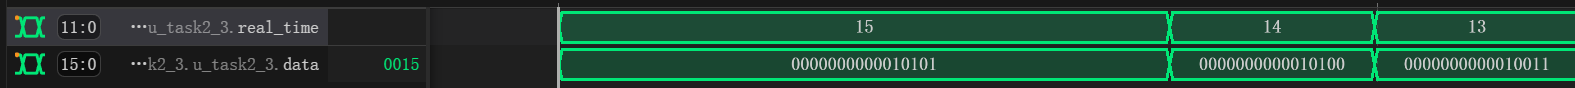
\includegraphics[width=0.8\textwidth]{task2_3_1.png}
    \caption{数据处理模块仿真}
\end{figure}
第一个信号比后面长的原因是正在reset。
\subsection{仿真设计}
代码如下,结果已经给出。
\begin{framed}
    \begin{lstlisting}[language=verilog,style=verilogStyle]
//~ `New testbench
`timescale 1ns/1ps
`include "task2_3.v"
module tb_task2_3;

    // task2_3 Parameters
    parameter PERIOD = 10;

    // task2_3 Inputs
    reg clk = 0;
    reg reset = 0;

    // task2_3 Outputs
    wire clk_div;
    wire buzz;
    wire [3:0] digit;
    wire [7:0] segment;

    task2_3 u_task2_3 (
        .clk(clk),
        .reset(reset),
        .clk_div(clk_div),
        .buzz(buzz),
        .digit(digit[3:0]),
        .segment(segment[7:0])
    );

    initial begin
        $dumpfile("./wave/tb_task2_3.vcd");
        $dumpvars(0, tb_task2_3);
        clk = 0;
        reset = 1;
        #10
        reset = 0;
        #10000
        $finish;
    end

    always begin
        #0.1 clk = ~clk;
    end

endmodule
    \end{lstlisting}
\end{framed}
\section{task2\_4}
\subsection{模块设计}
task2\_4相较于task2\_3只多一个计时控制模块,下面给出,其余模块相同,不再给出。
\subsubsection{计时控制模块}
\subsubsubsection{模块代码}
\begin{framed}
    \begin{lstlisting}[language=verilog,style=verilogStyle]
always @(posedge clk, posedge reset) begin
    if(reset) begin
        real_time = switch_io;
        data[3:0] = ((real_time)%60)%10;
        data[7:4] = ((real_time)%60)/10;
        data[11:8] = ((real_time)/60)%10;
        data[15:12] = ((real_time)/60)/10;
        buzz_flag <= 1'b0; 
    end
    else if(cnt == `CNT_MAX-1) begin
        if(real_time == 8'd0) begin
            buzz_flag = 1'b1;
            if(stop_flag == 1'b1) begin
                buzz_flag = 1'b0;
            end
        end
        else begin
            real_time = real_time - 8'd1;
            data[3:0] = ((real_time)%60)%10;
            data[7:4] = ((real_time)%60)/10;
            data[11:8] = ((real_time)/60)%10;
            data[15:12] = ((real_time)/60)/10;
        end
    end
end
    \end{lstlisting}
\end{framed}
第三行为该模块关键,上个模块\texttt{real\_time}为固定值,此时通过拨码开关控制。
\subsubsubsection{模块仿真}
\begin{figure}[H]
    %两张图并排,共用标题
    \centering
    \subfigure[image 1]{
        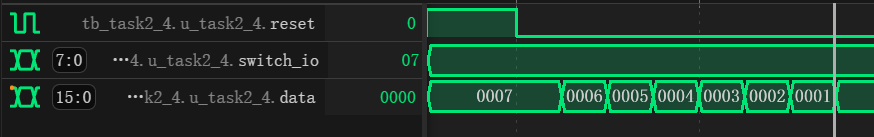
\includegraphics[width = 0.8\textwidth]{task2_4_1.png}
    }
    \subfigure[image 2]{
        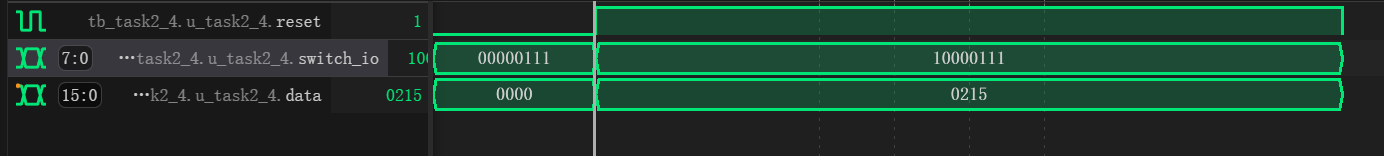
\includegraphics[width = 0.8\textwidth]{task2_4_2.png}
    }
    \caption{计时控制模块仿真}
\end{figure}
\subsection{仿真设计}
代码如下,结果已经给出。
\begin{framed}
    \begin{lstlisting}[language=verilog,style=verilogStyle]
//~ `New testbench
`timescale 1ns/1ps
`include "task2_4.v"

module tb_task2_4;

    // task2_4 Parameters
    parameter PERIOD = 10;

    // task2_4 Inputs
    reg clk = 0;
    reg reset = 0;
    reg [7:0] switch_io = 0;

    // task2_4 Outputs
    wire clk_div;
    wire buzz;
    wire [3:0] digit;
    wire [7:0] segment;

    task2_4 u_task2_4 (
        .clk(clk),
        .reset(reset),
        .switch_io(switch_io[7:0]),
        .clk_div(clk_div),
        .buzz(buzz),
        .digit(digit[3:0]),
        .segment(segment[7:0])
    );

    initial begin
        $dumpfile("./wave/tb_task2_4.vcd");
        $dumpvars(0, tb_task2_4);
        clk = 0;
        reset = 1;
        switch_io = 8'b00000111;
        #10
        reset = 0;
        #10000
        switch_io = 8'b10000111;
        reset = 1;
        #10
        reset = 0;
        $finish;
    end

    always begin
        #0.1 clk = ~clk;
    end

endmodule
    \end{lstlisting}
\end{framed}
\end{document}